\documentclass[12pt,a4paper,hidelinks]{report}
\usepackage{amsmath,amsthm,amssymb,graphicx,hyperref,mathptmx}
\usepackage[left=1.2in,right=1in,top=1in,bottom=1in]{geometry}
\usepackage[romanian]{babel}
\usepackage{float}
%\usepackage{...insert other packages here...}
\newtheorem{thm}{Teorema}[section]
\newtheorem{lem}[thm]{Lema}
\newtheorem{cor}[thm]{Corolarul}
\newtheorem{prop}[thm]{Propozi\c tia}
\theoremstyle{definition}
\newtheorem{defn}{Defini\c tia}[section]
\theoremstyle{remark}
\newtheorem{rem}{Remarca}[section]
\newtheorem{exmp}{Exemplul}[section]
\begin{document}
\thispagestyle{empty}
\begin{center}
\begin{figure}[h!]
\vspace{-20pt}
\begin{center}

\includegraphics[width=100pt]{images/FMI-03.png}
\end{center}
\end{figure}


{\large{\bf UNIVERSITATEA DE VEST DIN TIMI\c SOARA

FACULTATEA DE MATEMATIC\u A \c SI INFORMATIC\u A

PROGRAMUL DE STUDII DE LICEN\c T\u A: INFORMATIC\u A APLICAT\u A}}

\vspace{120pt}
{\huge {\bf LUCRARE DE LICEN\c T\u A}}

\vspace{150pt}
\end{center}

{\large\noindent{\bf COORDONATOR:\hfill ABSOLVENT:}

\noindent Conf. Dr. Forti\c s Florin \hfill Vidican Vlad-George}

\vfill
\begin{center}
{\bf TIMI\c SOARA

2023}
\end{center}
\newpage
\thispagestyle{empty}
\begin{center}
{\large{\bf UNIVERSITATEA DE VEST DIN TIMI\c SOARA

FACULTATEA DE MATEMATIC\u A \c SI INFORMATIC\u A

PROGRAMUL DE STUDII DE LICEN\c T\u A: INFORMATIC\u A APLICAT\u A}}

\vspace{120pt}
%{\huge {\bf LUCRARE DE LICEN\c T\u A/DIZERTA\c TIE}}
{\huge {\bf ThesisHub: Platforma web pentru lucr\u ari de licen\c t\u a/Dizerta\c tie}}

\vspace{150pt}
\end{center}

{\large\noindent{\bf COORDONATOR:\hfill ABSOLVENT:}

\noindent Conf. Dr. Forti\c s Florin \hfill Vidican Vlad-George}

\vfill
\begin{center}
{\bf TIMI\c SOARA

2023}
\end{center}
\newpage
\normalsize{}
\tableofcontents
\newpage
\chapter{Introducere}
\addcontentsline{toc}{chapter}{Introducere}

\section{Descrierea problemei}
Tema aleasă de către mine constă în dezvoltarea unei platforme online destinată studenților în anii terminali la unul dintre ciclurile de învățământ superior și profesorilor universitari în scopul coordonări sau găsirii unui coordonator pentru elaborarea lucrării de licența sau dizertație. Principalul mod în care platforma în cauză își propune să ajute în această privința este prin a facilita comunicarea dintre studenți și profesori, utilizatorii având posibilitatea de a-și posta propriile propuneri de teme sau de a aplica pentru unele din cele disponibile si active în acel moment, reducând astfel potențialul timp mort apărut pentru student în momentul aplicării pentru propuneri de teme a căror disponibilitate nu le este încă cunoscută dar și reducând comunicarea redundantă de ambele parți, propunerile având o secțiune de comentarii unde se pot acoperi eventualele întrebări frecvente.
\chapter{Solutii Similare}
\addcontentsline{toc}{chapter}{Solutii similare}
\section{Servicii de consultanta}
\subsection{Gradcoach}
\textbf{\textit{Gradcoach}} \footnote[1]{https://gradcoach.com/services/} este o platformă online care oferă suport contra cost studenților în realizarea lucrării de licența/dizertație, suportul variază în funcție de planul ales putând presupune:
\begin{itemize}
    \item Consiliere one-on-one cu un mentor specialist în domeniul temei alese. În timpul întâlnirii se pot discută: progresul, eventuale puncte de blocare și sugestii de îmbunătățire.
    \item Crearea și distribuirea de chestionare. colectarea și compilarea acestor răspunsuri. Transcripție în cazul în care datele colectate vin în format audio sau audio-video și codarea datelor.
    \item Ajustări pentru variantă finală a lucrării, cum ar fi repararea greșelilor gramaticale, asigurarea consecvenței și respectării standardelor universității în ceea ce privește redactarea lucrării (font, spațiere, cuprins, citate și referințe, numerotarea paginii).
\end{itemize}




\subsection{ThesisHelpers}
\textbf{\textit{Thesishelpers}}\footnote[2]{https://www.thesishelpers.com/about} este o platformă online similară cu gradcoach, în sensul că și aceasta oferă servicii studenților pentru realizarea lucrării de licența/dizertație, aceste servici fiind: 
\begin{itemize}
    \item Ajustări pentru varianta finală a lucrării.
    \item Editare ușoara (restructurarea textului, rescrierea anumitor propoziții pentru o alegere mai bună a cuvintelor păstrând însă ideea din spate intactă).
    \item Realizarea întregi lucrări, clientul fiind responsabil doar de setarea cerințelor pentru această lucrare.
\end{itemize} 
\subsection{Compara\c tie}
Soluția mea este diferită față de cele două platforme menționate mai sus, deoarece aceasta va fi o platformă internă, non-profit care își propune doar să faciliteze comunicarea dintre studenți și profesori în scopul realizării lucrării necesare pentru absolvirea ciclului de studiu ales în timp ce platformele menționate mai sus oferă servicii contra cost a unor consultanți externi, unele dintre aceste servicii presupunând chiar plagiarism și implicit încălcarea integrității academice
\section{Platforme de matchmaking}
O platformă de matchmaking are ca scop fundamental potrivirea de persoane. Matchmaking-ul este un termen-umbrelă destul de vast, care acoperă o multitudine de servicii/platforme, toate aceste servicii având însă ca scop potrivirea unei persoane care are o problemă/nevoie cu o persoană care poate oferi o soluție. În cazul de față, platforma dezvoltată de mine poate fi considerată o platformă de matchmaking, deoarece potrivește studenți care au nevoie de consiliere în scopul realizării unei lucrări de licența/dizertație cu un profesor coordonatorcare poate oferi această consiliere.
Cateva astfel de exemple sunt:
\subsection{Fiverr}
\textbf{\textit{Fiverr}}\footnote[1]{https://www.fiverr.com} este o platforma web in care utilizatorii au posibilitatea de a posta servicii pe care aceștia le oferă (ex: proof-reading, voice-over, colectare de date, etc) și prețurile pe care le cer pentru aceste servicii.
\subsection{Freelancer}
\textbf{\textit{Freelancer}} \footnote[2]{https://www.freelancer.com/jobs} este o platforma pe care utilizatorii postează proiecte în care detaliază serviciile de care au nevoie și un preț maxim pe care sunt dispuși să îl plătească pentru acel serviciu, iar ceilalți utilizatori pot licită pentru acel proiect (concurând cu ceilalți utilizatori care doresc să preia acel proiect prin prețuri cât mai competitive).
\subsection{MentorNet}
\textbf{\textit{MentorNet}} \footnote[3]{https://greatmindsinstem.org/mentornet/} este o organizație non-profit care își propune să pună studenți în contact cu specialiști în domeniul acestora de studiu pentru dezvoltarea unei relații de mentorat. După procesul inițial de asociere a unui student cu un mentor, aceștia vor purta discuții săptămânale  pentru a discută despre proiecte, planuri de carieră, și alte topicuri relevante pentru viitorul studentului.
\subsection{Comparatie}
Platforma dezvoltată de mine se deosebește de primele două exemple, deoarece nu este concepută ca o piața de desfacere pentru servicii. S-ar putea ca unii utilizatori să ofere servicii de consultanță asemănătoare cu \textbf{\textit{Gradcoach}} sau \textbf{\textit{Thesishelpers}} pe aceste platforme, dar în esența acestea se aseamănă doar prin faptul că sunt platforme de matchmaking.

Există o asemănare mai puternică însă între \textbf{\textit{MentorNet}} și platforma dezvoltată de mine, deoarece ambele au ca scop fundamental să faciliteze stabilirea unor relații de mentorat în folosul studenților, platforma mea diferențiindu-se de către aceasta prin specificul său. \textbf{\textit{MentorNet}} își asumă o abordare generalistă asupra mentoratului și oferă astfel doar sistemul de matchmaking, care permite inițierea relației de mentorat și un mijloc de comunicare. În schimb, platforma aceasta este concepută în jurul realizării lucrării de licența/dizertație, oferind astfel facilitați care să asiste în acest proces. Aceasta este de asemenea concepută drept o platformă internă spre deosebire de \textbf{\textit{MentorNet}}, accesul fiind astfel oferit doar profesorilor și studenților din aceeași universitate, lucru garantat prin faptul că administratorii platformei sunt responsabili de integrarea noilor utilizatori, aceștia fiind nevoiți să atașeze dovezi de identitate odată cu cererea de creare a unui cont, cerere care va fi ulterior validată de un administrator.
\chapter{Arhitectura si facilitățile aplicației}
\section{Cazuri de utilizare pentru utilizatorii standard}
\begin{figure}[h]
    \centering
    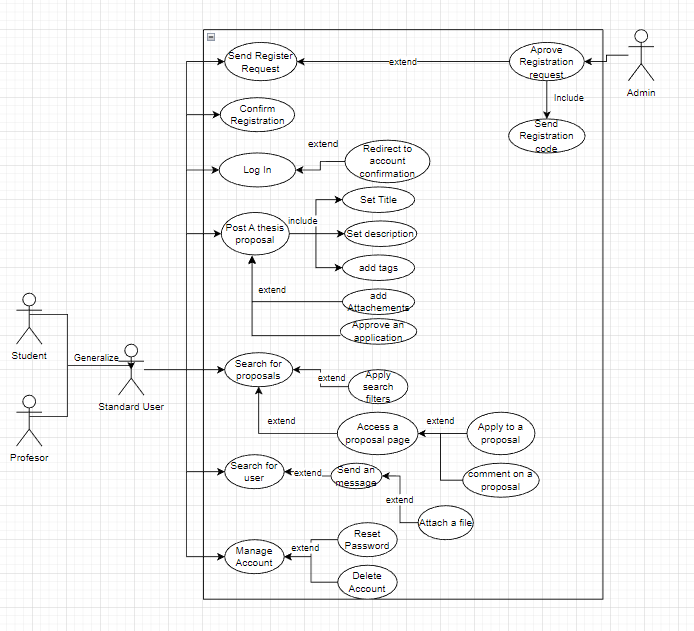
\includegraphics[scale=0.5]{images/StandardUserUseCase.png}
    \caption{Cazuri de utilizare pentru utilizatorii standard}
    \label{fig:stdUserDiagram}
\end{figure}
În diagrama de mai sus am ales să generalizez utilizatorul de tip Student și utilizatorul de tip Profesor ca un actor de tip „Utilizator standard” dat fiind faptul ca facilitățile disponibile celor  două tipuri de conturi sunt aceleași, diferențierea dintre cele două tipuri de conturi fiind totuși necesară din punct de vedere semantic(nu ar avea sens ca aplicația să permită unui student să coordoneze lucrări, sau unui profesor să aplice pentru tema propusă de alt profesor). Am încercat să cuprind în această diagramă toate cazurile de utilizare disponibile  unui utilizator standard cu scopul de a avea o imagine generala asupra facilitaților oferite de către platforma, voi analiza detaliat însă publicarea pe platforma a unei noi propunere de lucrări:



Acest caz de utilizare descrie procesul prin care noile propuneri de lucrări sunt adăugate pe platforma
\begin{itemize}
    \item{Actorii:
        \begin{enumerate}
            \item Utilizator standard
        \end{enumerate}}
    \item{Precondi\c tii:
        \begin{enumerate}
            \item Utilizatorul este de tip Profesor sau Student
            \item Contul acestuia trebuie să fi trecut atât de aprobarea înregistrării de către un administrator al platformei cât și confirmarea acesteia de către utilizator
            \item Utilizatorul este autentificat pe platformă
        \end{enumerate}}
    \item{Scenariu:
        \begin{enumerate}
            \item Accesarea paginii pentru crearea unei propuneri de licență
            \item Introducerea unui Titlu
            \item Introducerea unei Descrierii
            \item {Selectarea etichetelor potrivite temei propuse din lista de etichete disponibile
                \begin{enumerate}
                    \item utilizatorul este nevoit să selecteze cel puțin o etichetă pentru a continua
                \end{enumerate}}
            \item Opțional: Adăugarea eventualelor atașamente utile pentru descrierea temei propuse celorlalți utilizatorii interesați
            \item Dacă oricare dintre câmpurile menționate mai sus este invalid (gol sau prea scurt) atunci utilizatorul este avertizat
            \item Noua propunere de lucrare este creata pe platformă
        \end{enumerate}}
    \item{Postcondi\c tii:
        \begin{enumerate}
            \item Noua propunere este adăugată în baza de date a platformei și devine vizibilă celorlalți utilizatori ai platformei, ei putând interacționa cu această
        \end{enumerate}}
\end{itemize}
\section{Cazuri de utilizare pentru administratori}
\begin{figure}[H]
    \centering
    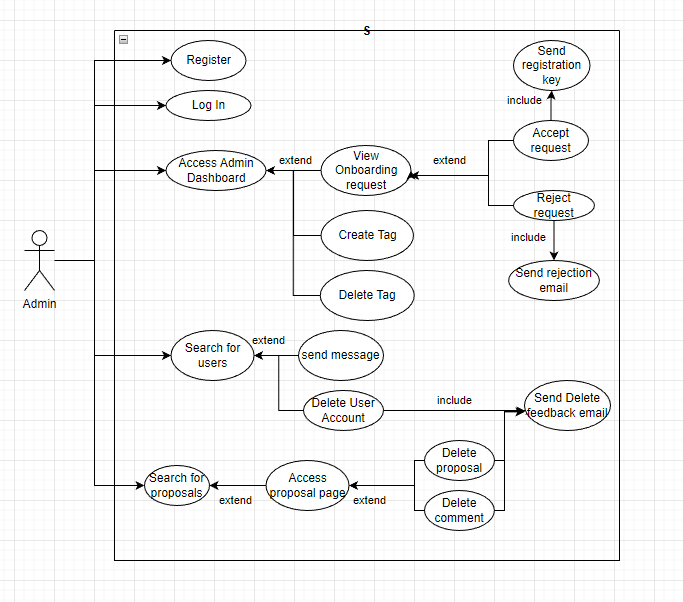
\includegraphics[scale=0.5]{images/AdminUserUseCase.png}
    \caption{Cazuri de utilizare pentru Administratori}
    \label{fig:adminUseCaseDiagram}
\end{figure}
Administratorii sunt utilizatorii cu privilegii ridicate, care au posibilitatea și responsabilitatea să gestioneze accesul celorlalți utilizatorii la platformă și să modereze conținutul acesteia pentru a păstra calitatea conținutului platformei la standardele universității și a unui mediu academic (eliminarea potențialelor postări/comentarii inadecvate scopului platformei), acest tip de conturi este gândit ca unul strict administrativ neavând astfel capacitatea de a:
\begin{itemize}
    \item Publica propuneri de lucrări.
    \item A aplica pentru propunerile existente sau de a lasă comentarii asupră acestora.
\end{itemize}
funcționalitățile comune cu conturile de utilizator standard fiind doar:
\begin{itemize}
    \item Autentificarea.
    \item Căutarea și accesarea  propunerilor de lucrări de pe platformă.
    \item Trimiterea de mesaje celorlalți utilizatori.
\end{itemize}
Am ales de asemenea că pentru diagramă de mai sus să abstractizez funcționalitatea ce ține de autentificare și trimiterea de mesaje, această fiind identică cu cea a conturilor standard reprezentate deja mai detaliat în diagrama precedentă, mai jos se poate revedea o analiză mai în detaliu a cazului de utilizare pentru aprobarea sau respingerea unei cererii de înregistrare.
\begin{itemize}
    \item {Actorii:
        \begin{enumerate}
            \item Administrator.
        \end{enumerate}}
    \item {Precond\c tii:
        \begin{enumerate}
            \item Utilizatorul are un cont de administrator pe platformă.
            \item Contul acestuia trebuie să fii trecut atât de aprobarea înregistrării de către un administrator al platformei cât și confirmarea acestuia de către utilizator.
            \item Utilizatorul este autentificat pe platformă.
            \item Există cel puțin o cerere de înregistrare pe platformă.
        \end{enumerate}}
    \item {Scenariul standard:
        \begin{enumerate}
            \item Utilizatorul accesează bordul de gestionare al administratorilor.
            \item Utilizatorul alege una dintre cererile de înregistrare.
            \item Utilizatorul verifica datele afișate in cererea de înregistrare.
            \item Utilizatorul verifica dovezile de identitate atașate de persoana care a inițiat cererea.
            \item Utilizatorul validează cererea.
            \item un email automat va fii trimis de către sistem utilizatorului care a inițiat cererea conținând un cod necesar pentru confirmarea înregistrării.    
        \end{enumerate}}
    \item {Postcondi\c tii:
        \begin{enumerate}
            \item Cererea o dată procesată va dispărea din bordul de gestionare al administratorilor.
            \item Un cod de confirmare a înregistrării este generat de către sistem și primit de către persoana care a inițiat cererea pe adresa de email folosită de către aceasta la crearea contului.
            \item Utilizatorul care a inițiat cererea are acum potențialul de își confirma contul, având apoi acces la restul funcționalităților de pe platformă.
        \end{enumerate}}
    \item {Scenariu alternativ:
        \begin{enumerate}
            \item Utilizatorul accesează bordul de gestionare al administratorilor.
            \item Utilizatorul alege una dintre cererile de înregistrare.
            \item Utilizatorul verifică datele afișate în cererea de înregistrare.
            \item Utilizatorul verifică dovezile de identitate atașate de persoana care a inițiat cererea.
            \item Utilizatorul respinge cererea.
            \item Utilizatorul este nevoit să justifice decizia de a respinge cererea.
            \item Un email de informare împreună cu justificarea respingerii oferită de către administratorul care a procesat cererea respectivă este trimis.
        \end{enumerate}}
    \item {Postcondi\c tii:
        \begin{enumerate}
            \item Cererea o dată procesată vă dispărea din bordul de gestionare al administratorilor.
            \item Contul nu a fost creat și un email de informare a fost trimis de către sistem.
        \end{enumerate}}
\end{itemize}
\section{Design-ul bazei de date}
\subsection{Privire de ansamblu}
\begin{figure}[H]
    \centering
    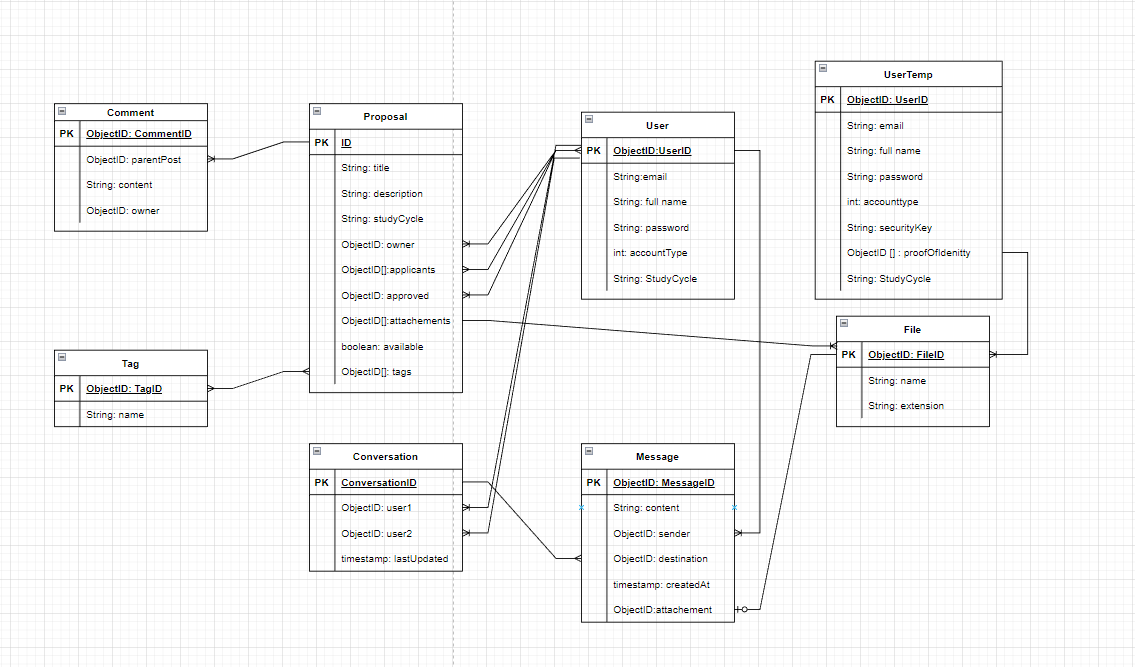
\includegraphics[scale=0.4]{images/DB_Diagram.png}
    \caption{Diagrama bazei de date}
    \label{fig:dbDiagram}
\end{figure}
Pentru dezvoltarea acestei platforme am ales să folosesc MongoDB ca și sistem de gestionare a bazelor de date(DBMS). Acesta este un DBMS de tip NoSQL, bazat pe documente (echivalentul rândurilor într-o baza de date de tip SQL) și colecții (echivalentul tabelelor în baze de date SQL), documentele sunt scrise în format BSON(Binary Javascript Object Notation), Acest format suportând obiecte(imbricarea obiectelor fiind suportată de asemenea) și vectorii de valorii primitive sau de obiecte pe lângă tipurile primitive comune cu SQL, Acest fapt oferă o flexibilitate semnificativ mai mare în proiectarea unei baze de date spre deosebire de un DMBS de tip  SQL, această flexibilitate vine însă la costul consistenței, o colecție nu impune în mod nativ o schemă asupră documentelor pe care le are în apartenentă, astfel în mod teoretic se poate ca două documente din aceiași colecție sa conțină o structură si/sau atribute diferite, de regulă sunt impuse însă soluții de validare a operațiunilor de creare/modificare pentru a putea asigura o consecvența a datelor.

Mai jos se poate regăsii o scurta descriere a fiecărei colecții regăsite în diagrama de mai sus
\subsection{Analiza colec\c tiilor din baza de date}
\subsubsection{User}
În această colecție vor fi stocate toate documentele care conțin informații despre utilizatorii aplicației, informații precum:
\begin{itemize}
    \item Nume.
    \item Email.
    \item Parola.
    \item Tip de utilizator (Profesor, Student sau Administrator).
    \item Ciclu de studiu(Licen\c ta sau Master)    
\end{itemize}
parolele sunt de asemenea trecute printr-un algoritm de „hashing”\footnote[1]{ in acest context un proces unidirectional si determinist de a mapa un \c sir de caractere la unul nou, de lungime fixa si cu un aspect complet aleatoriu pentru un eventual actor malitios care a ob\c tinut access la baza de date} înainte de a fii stocate din motive de securitate.
\subsubsection{UserTemp}
În această colecție sunt stocate cererile de înregistrare pe platformă, pe lângă câmpurile din colecția „User” avem un câmp în plus care va stoca o cheie de confirmare și referințe către dovezile de identitate aferente cererii din colecția de fișiere, în momentul când utilizatorul creează o cerere de înregistrare pe platformă un document nou va fii creat în această colecție având câmpul cheii de confirmare nul, o dată validată cererea de către administrator o cheie de confirmare va fii generată pentru acest utilizator și transmisă acestuia prin email, odată cu confirmarea înregistrării de către utilizator folosind cheia primită un document nou va fii creat în colecția "User" iar cel aferent cererii de înregistrare va fii șters din colecția „UserTemp”.
\subsubsection{Comment}
În această colecție sunt stocate comentariile de pe platformă, pe lângă conținutul comentariului se mai stochează și o refererin\c ta către utilizatorul care a postat comentariul și către propunerea de tema asupra căreia a fost lasat comentariul.
\subsubsection{Tag}
În aceasta colecție se găsesc etichetele pe care un utilizator le poate atașa unei propuneri la creare, ștergerea și adăugarea de documente noi în aceasta colecție este rezervată exclusiv administratorilor
\subsubsection{Conversation}
Această colecție servește funcționalita\c tii de mesagerie a platformei, aici sunt stocate conversațiile (doar membrii, nu și conținutul) de pe platformă, împreuna cu o data care reprezintă data și timpul ultimului mesaj nou în aceea conversație(necesar pentru afișarea conversațiilor unui utilizator în ordine cronologică.
\subsubsection{Message}
Această colecție stochează mesajele trimise de către utilizatorii, atributul „sender” conține id-ul utilizatorului care a trimis mesajul iar cel de „destination„ conține id-ul conversației în care a fost trimisă, utilizatorul   care doreste sa trimita un mesaj nou trebuie evident să fie un membru al acelei conversații.
\subsubsection{File}
Această colecție stochează numele fișierelor aferente platformei și extensia acestora, fișierele în sine fiind stocate în sistemul de fișiere al serverului, această colecție stocând doar referințe către acestea.
\subsubsection{Proposal}
această colecție stochează propunerile de teme de pe platformă, aceasta deține câmpuri primitive precum:
\begin{itemize}
    \item Descriere.
    \item Titlu.
    \item Ciclu de studiu.
    \item Disponibilitate.
\end{itemize}
dar și referințe către alte colecții precum:
\begin{itemize}
    \item "owner” reprezintă id-ul utilizatorului care a publicat propunerea de tema.
    \item „applicants” reprezintă un vector de id-uri ale unor utilizatori care au aplicat pentru propunerea în cauză.
    \item „attachaments” un vector de id-uri către fișierele aferente propunerii.
    \item „tags” conține referințe către etichetele atașate propunerii.
    \item „approved” conține o referința către utilizatorul a cărui aplicație a fost aprobată de către „owner” această referința este nula la creare și rămâne așa până când o aplicație este aprobată.
\end{itemize}
%\bibliography{mybib}
%\bibliographystyle{alpha}
%\addcontentsline{toc}{chapter}{Bibliography}
\end{document} 